\documentclass[10pt,a4paper]{article}
\usepackage[utf8]{inputenc}
\usepackage[english]{babel}
\usepackage{amssymb,amsfonts, amsmath}
\usepackage{graphicx}
\usepackage{listings, color}
\usepackage{url}
\usepackage{float}


\title{\rule{12.5cm}{0.5mm}\\Advanced Algorithms in Computational Biology\\DM845}
\author{Martin Østergaard Villumsen\\\texttt{mvill11@student.sdu.dk}\\\rule{6.5cm}{0.5mm}\\University of Southern Denmark\\}
\date{\today}

\begin{document}
\maketitle
\newpage

\section{Introduction}
The human genome is diploid which means that each cell has two homologous copies of each chromosome, one from the mother and one from the father. In order to understand the genetic basis for different diseases (e.g. cancer) it is not sufficient to detect the SNPs, we also need to assign each SNP to the two copies of the chromosome and current methods for doing so suffers from the fact that the reads are too short \cite{whatshap}.

In this project we will develop a simple read simulator, which generates reads that are much longer than those obtained from e.g. Next-Gen sequencing machines. We will simulate reads with different parameters such as read length and sequencing error probability and assign SNPs to each chromosome from these reads using \textsc{WhatsHap}, a novel dynamic programming approach to haplotype assembly described in \cite{whatshap}. We will then evaluate the results and compare them with those presented in \cite{whatshap}.

\subsection{Biological Problem}
The task of assigning SNPs to a concrete chromosome is called phasing and the resulting groups of SNPs are called haplotypes. We need to discover and phase all these SNPs in order to gain a better understanding for e.g. some diseases by linking possibly disease-causing SNPs with one another. By doing so we can reconstruct haplotypes from a collection of sequenced reads which is known as haplotype assembly.

\subsection{Computational Problem}
There are two groups of single nucleotide variants: Those that are homozygous and those that are heterozygous. Individuals that are homozygous at every locus or heterozygous at just one locus can easily be phased, however, if we have $m$ heterozygous SNPs, there are $2^m$ possible haplotypes which illustrates that it is a hard computational problem. Therefore we are only concerned with heterozygous SNPs when doing haplotype assembly. 

What also makes this a computational hard problem is the fact that we want to phase an reconstruct the haplotypes directly from sequencing reads. 

\section{Haplotype Assembly with WhatsHap}
There are two major approaches to phasing variants: One approach relies on genotypes as input along with the zygosity status of the SNPs, and the other approach phases directly from sequencing read data \cite{whatshap}. \textsc{WhatsHap} belongs to the latter. 

\textsc{WhatsHap} has been developed with the parsimony principle in mind, i.e. computing two haplotypes to which we can assign all reads while minimizing the amount of sequencing errors to be corrected or removed \cite{whatshap}. This resembles the minimum error correction (MEC) problem which consists of finding the minimum number of corrections to the SNP values to be made to the input in order to be able to arrange the reads into two haplotypes without conflicts \cite{whatshap}. This can easily be adapted to a weighted version of the problem, namely the weighted minimum error correction problem (wMEC). The weight in this case reflects the relative confidence that a single nucleotide is correctly sequenced.

Even though the wMEC problem is NP-hard \textsc{WhatsHap} creates an exact solution to the problem in linear time. This is done by the use of dynamic programming and assuming a bounded coverage, i.e. the implementation can solve the problem in linear time on datasets of maximum coverage up to 20x \cite{whatshap}. The algorithm is a fixed parameter tractable approach to the wMEC where the running time is only depending on the coverage, i.e. the number of reads that cover a SNP position.

The input to the wMEC problem is a matrix with entries $\in\{0, 1, -\}$ where each row corresponds to a read and each column corresponds to a SNP position. Each entry is associated with a weight telling how likely it is that the entry is correctly sequenced. We want to find a minimum weight solution and when these weights are log-likelihoods, summing them up corresponds to multiplying probabilities, thus finding the minimum weight solution corresponds to finding a maximum likelihood bipartition of the reads \cite{whatshap}. And this is basically what the authors of \textsc{WhatsHap} is using a dynamic programming approach to do. By using this approach they find an optimal solution to the wMEC problem for each column of the matrix and then an optimal bipartition of the reads can be obtained by backtracking along the columns of the dynamic programming table. See \cite{whatshap} for further details.

The implementation of \textsc{WhatsHap} can be found at \url{https://bitbucket.org/whatshap/whatshap} and the documentation can be found at \url{https://whatshap.readthedocs.org/en/latest/}. The software requires a \texttt{VCF}-file and a \texttt{BAM}-file as input. \texttt{VCF}-files describe gene sequence variations, i.e. a list of variants and genotypes for the diploid genome, and \texttt{BAM}-files are the compressed binary equivalent of \texttt{SAM}-files, which are \textit{Sequence Alignment/Map}-files that contain sequence data in a series of tab delimited ASCII columns, i.e. aligned reads for the individual diploid genome that are coordinate sorted (i.e. by chromosal position).
% Description of data

\section{Building a DNA Simulator}
There already exists different DNA read simulators but for this project we decided to design and implement our own simple simulator to generate data for \textsc{WhatsHap}. The lecturer of the course has provided a reference chromosome (\texttt{chr1.fa}) which we have used as a basis for the simulation of DNA reads. The chromosome is in \texttt{FASTA}-format (\texttt{.fa}) which is a text-based format for representing nucleotide sequences.

For this implementation we have used \texttt{Python 2.7.9}. Also, for this implementation we assume that there are no \texttt{N}s in the chromosome, i.e. the \texttt{N}s present in \texttt{chr1.fa} are removed and the only letters present are: \texttt{A, T, C, G}.

\subsection{Generating a Chromosome with Mutations}
Before building the actual simulator we needed a script to generate a \texttt{VCF}-file describing the chromosome with mutations. Generating the \texttt{VCF}-file is done with a simple \texttt{Python} script that reads the chromosome, removes all \texttt{N}s (if there are any) and copy the chromosome one nucleotide at a time. Every 400 + 'random integer between 0-100' we simulate a mutation (i.e. a single nucleotide variant) by randomly choosing one of the remaining nucleotides. E.g. if the current nucleotide is \texttt{A} we randomly choose a nucleotide from \{\texttt{T, C, G}\}. For every simulated mutation a line is written to the \texttt{VCF}-file with the following values:
\begin{itemize}
\item CHROM: \texttt{'chr1'}
\item POS: The position of the nucleotide in the chromosome
\item ID: The position of the nucleotide in the chromosome
\item REF: The nucleotide from the reference chromosome
\item ALT: The "new" nucleotide (i.e. the variant)
\item QUAL: \texttt{'.'}
\item FILTER: \texttt{'PASS'}
\item INFO: \texttt{'.'}
\item FORMAT: \texttt{'GT'}
\item sample: \texttt{'0/1'}
\end{itemize}
This \texttt{VCF}-file can then be used to generate a copy of the chromosome with mutations which we will need for simulating the DNA reads.

See \texttt{buildVCF.py} for details on the implementation.

\subsection{Simulating DNA Reads}
There are two types of variants which can occur in DNA reads: Sequencing errors and mutations. We need to take both into account when designing a read simulator. Also, we need to be able to choose how many reads the simulator should generate, how long the reads should be and the percentage of sequencing errors that should occur in the simulated reads. This is all given as parameters to the program. We have designed the read simulator as follows:
\begin{enumerate}
\item Read the \texttt{FASTA}-file (reference chromosome) and the \texttt{VCF}-file (both are given as input) and remove line breaks, comments etc.
\item Generate a copy of the reference chromosome with mutation from the \texttt{VCF}-file.
\item Generate reads one at a time as follows:
\subitem a. Choose one of the two chromosomes at random.
\subitem b. Choose a random start position for the read.
\subitem c. Iterate over the next $x$ nucleotides, where $x$ is the read length.
\subitem d. For each nucleotide in the read, alter the nucleotide with probability $e$, where $e$ is the probability that a sequencing error occurs.
\item Repeat a. - d.  $r$ times where $r$ is the number of reads we want to generate.
\end{enumerate}
When all reads have been generated the program generates a \texttt{SAM}-file describing the reads, which is written to a file. We have chosen to leave out many of the values of the \texttt{SAM}-file to keep things simple. We have chosen to use the following header:
\begin{lstlisting}
@HD	VN:1.4	GO:none	SO:coordinate
@SQ	SN:chr1	LN:'length of chromosome'
@RG	ID:1	PL:Platform	LB:library	SM:sample
\end{lstlisting}
along with the following values for each line of the file:
\begin{itemize}
\item QNAME: \texttt{'r00\%d'} where '\%d' is the start position of the read in the reference chromosome
\item FLAG: \texttt{'0'}
\item RNAME: \texttt{'chr1'}
\item POS: 'Start position of the read in the reference chromosome'
\item MAPQ: '255' (this indicates that the value is not available)
\item CIGAR: \texttt{'\%dM'} where '\%d' is the length of the read
\item RNEXT: \texttt{'='}
\item PNEXT: \texttt{'0'}
\item TLEN: 'Length of the chromosome'
\item SEQ: 'The actual read'
\item QUAL: 'A string of length $r$ consisting of "J"s, where $r$ is the length of the read'
\end{itemize} 
For details about the individual field see the SAM Format Specification at \url{https://samtools.github.io/hts-specs/SAMv1.pdf}. For details about the implementation of the simulator see \texttt{sim.py}.

\subsection{How to Use the Simulator}
%% TODO: List of commands to recreate my results.

\section{Results and Discussion}
%% TODO: List of commands to recreate my results.
%% TODO: What parameters have been used.

\section{Conclusion}
% Why does it not work with 1.000.000 reads ??? Length of chrm1: 230.481.193


\addcontentsline{toc}{section}{References}
\bibliography{whatshap}{}
\bibliographystyle{abbrv}
\newpage
\appendix
\section{Figures}
\begin{figure}[!ht]
\centering
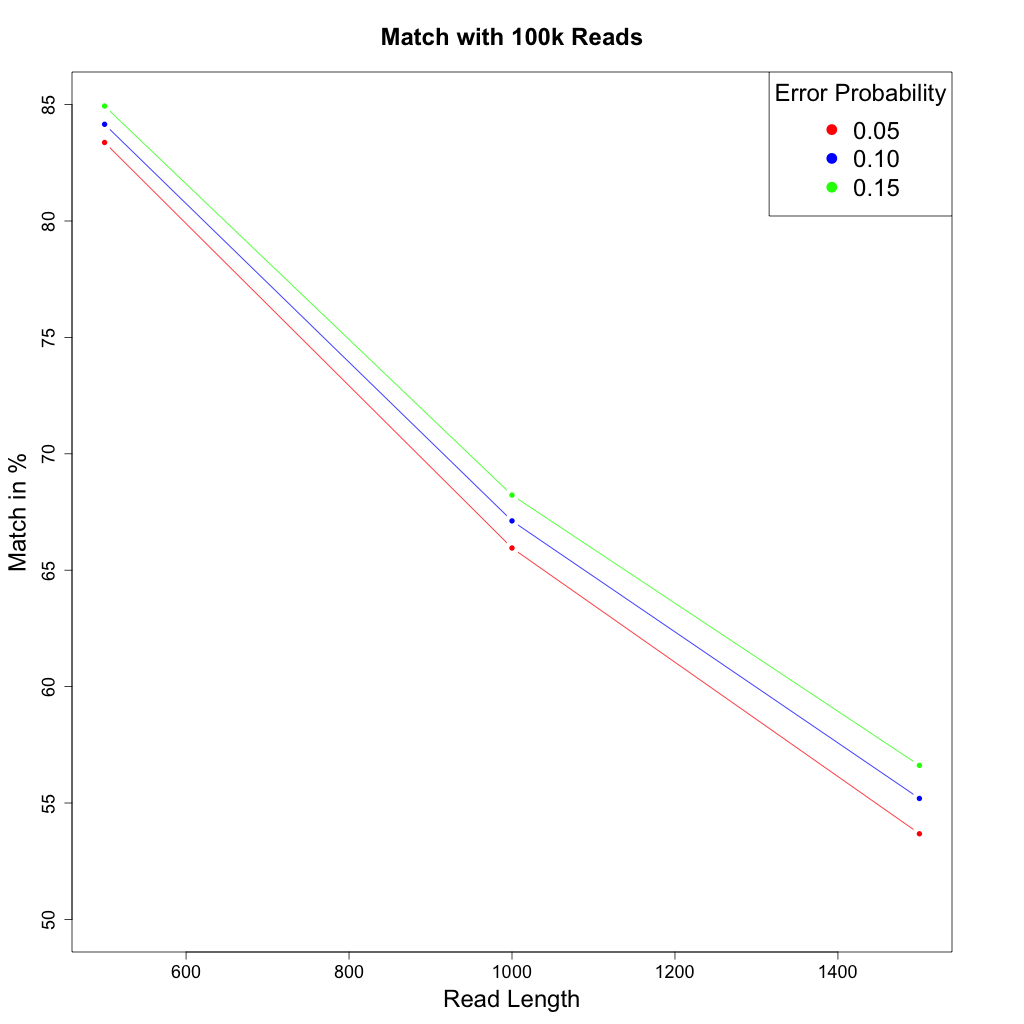
\includegraphics[height=0.4\textheight]{../output/plots/plot100k}
\caption{\footnotesize Results of haplotype assembly of 100.000 reads.}
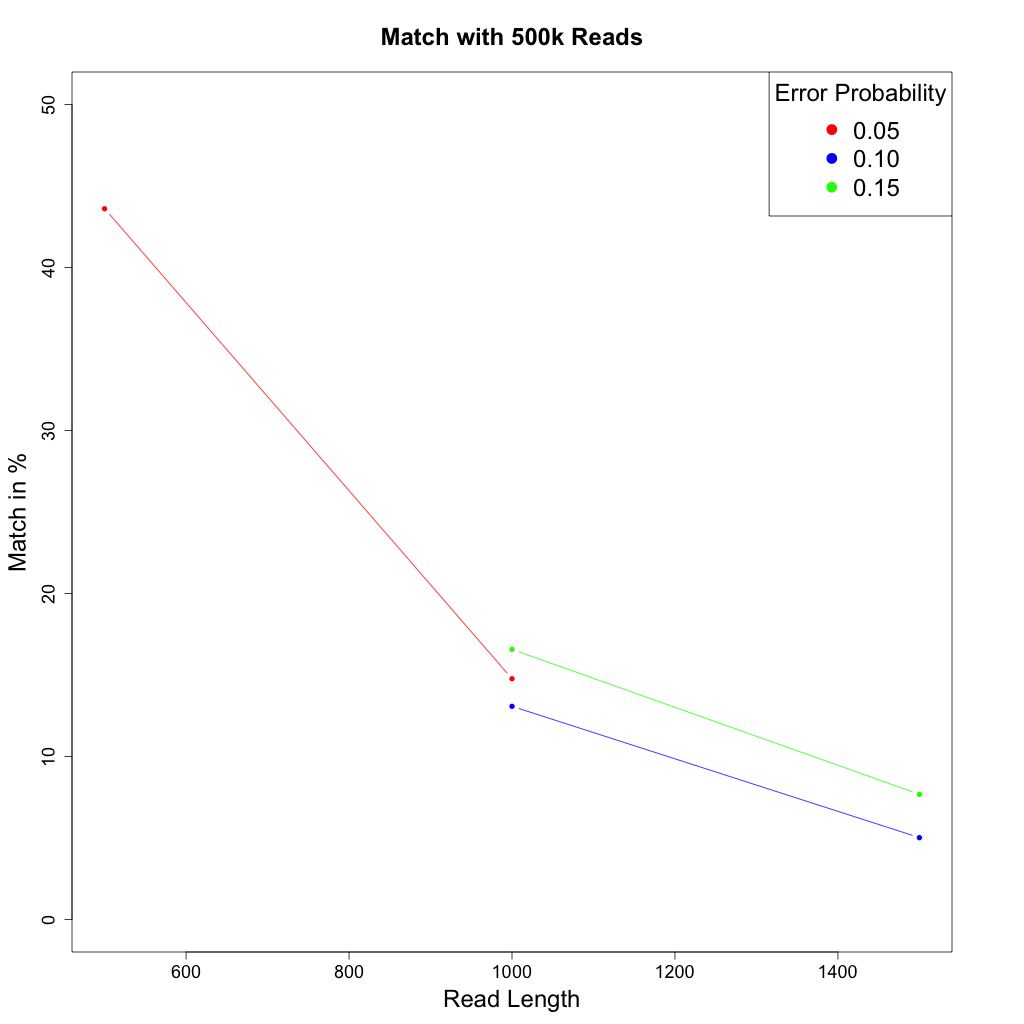
\includegraphics[height=0.4\textheight]{../output/plots/plot500k}
\caption{\footnotesize Results of haplotype assembly of 500.000 reads.}
\end{figure}
\newpage
\begin{figure}[!ht]
\centering
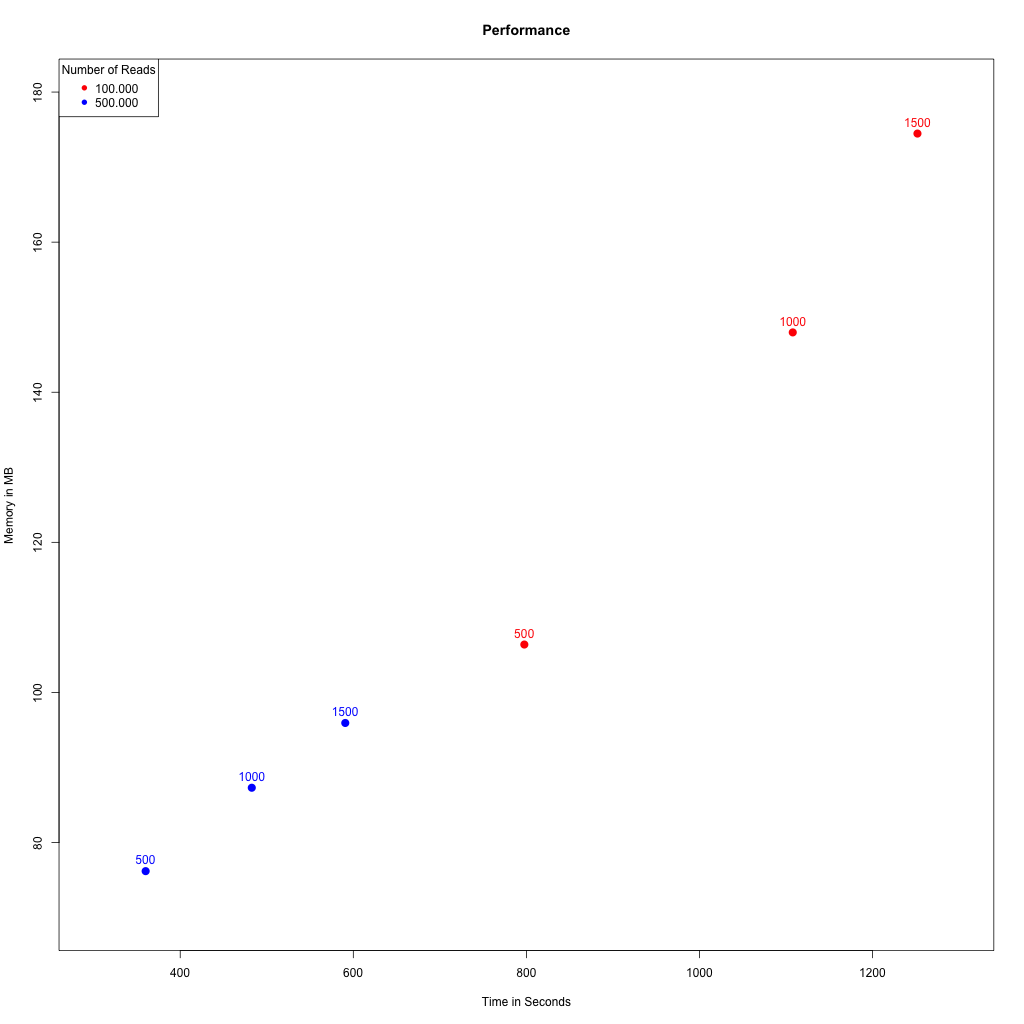
\includegraphics[width=\textwidth]{../output/plots/plotPerformance}
\caption{\footnotesize Performance measured in memory (in MB) and time (in sec.) and with two different number of reads.}
\end{figure}

\end{document}
